\subsection{Augmented State Machine}
\label{subsec:augment}

To deal with the inherent uncertainty of sniffer traces, we propose to
systematically augment the original checker state machine with non-deterministic
transitions to account for the difference between the sniffer and DUT traces.


\begin{figure}[t!]
  \centering
  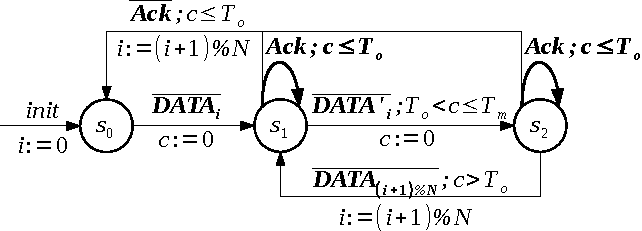
\includegraphics[width=0.48\textwidth]{./figures/dot11_tx_checker.pdf}
  \caption{\textbf{Augmented Checker State Machine.} Augmented transitions are
  highlighted in bold face. $\overline{Pkt}$ means either $\epsilon$ or $Pkt$.}
  \label{fig:augment}
\end{figure}


Before formally defining the augmented state machine, we first use an example to
illustrate the basic idea.
%
Figure~\ref{fig:augment} shows the augmented state machine
for 802.11 transmitter state machine shown in Figure~\ref{fig:dot11_tx_ta}.
%
For each existing transition (e.g., $s_0\rightarrow s_1$), we add an \textit{empty
transition} with same clock guards and resetting
clocks.
%
This is to account for the possibility when such packet was observed by
the DUT but missed by the sniffer.
%
Additionally, for each transition triggered
by a \textit{receiving} packet (i.e., $p.dest = DUT$), such as $s_1\rightarrow
s_0$ and $s_2\rightarrow s_0$, we add a \textit{self transition} with the same
trigger packet and clock guards, but empty set of resetting clocks.
%
The presence of this transition allows the protocol to make progress on a trace,
and not get stuck

There are two points worth noticing.
%
First, self transitions are added only for
receiving packets with respect to the DUT.
%
If the sniffer observes a sending packet from the DUT, then the packet must
also appear in the DUT's observation.
%
In other words, there is no uncertainty for such packets when they
are observed by the sniffer.
%
Second, no augmented transition are added for the packets that are sent to DUT yet
are missed by both the DUT and the sniffer, since such packets do not cause
difference between the DUT and sniffer traces.

The augmented state machine in Figure~\ref{fig:augment} will accept the sniffer
packet traces $Tr_1$ and $Tr_2$ shown in Figure~\ref{fig:sniffer_in_middle}.
%
For instance, one accepting transition sequence on sniffer trace $Tr_1$ is
$s_0\rightarrow s_1 \rightarrow_s s_1\rightarrow s_2 \rightarrow s_0$, and the
sequence for $Tr_2$ is $s_0 \rightarrow s_1 \rightarrow_e s_2 \rightarrow s_0$,
where $\rightarrow$ is the transition from the original state machine,
$\rightarrow_e$ and $\rightarrow_s$ are the augmented empty and self transitions
respectively.

We now formally define the augmented state machine.

\begin{definition}
  An augmented state machine $S^+$ for a checker state machine $S$ is a 6-tuple
  $\{\boldsymbol{\Sigma^+}, \mathbb{S}, s_0, C, \boldsymbol{E^+}, G\}$, where $\mathbb{S},
  s_0, C, G$ are the same with $S$. $\Sigma^+=\{\epsilon\} \cup \Sigma$ is
  the augmented input alphabet with the empty symbol, and $E^+ \supset E$ is the
  set of transitions, which includes:
  \begin{itemize}
    \item $E$: existing transitions (\textbf{Type-0}) in $S$.
    \item $E^+_1$: empty transitions (\textbf{Type-1}) for each transition in $E$.
    \item $E^+_2$: self transitions \textbf{(Type-2)} for each transitions
      triggered by receiving packets.
  \end{itemize}
\end{definition}

Algorithm~\ref{alg:augment} describes the process of transforming $E$ into
$E^+$.
%
In particular, Line~\ref{alg:augment:type0} adds existing transitions in $E$ to
$E^+$, while line~\ref{alg:augment:type1} and~\ref{alg:augment:type2} add Type-1
and Type-2 transitions to $E^+$ respectively.

\begin{algorithm}[t!]
  \begin{algorithmic}[1]
    \Function{augment}{$E$}
    \Let{$E^+$}{$\emptyset$}
    \ForAll{$\langle s_i, s_j, p, g, C'\rangle \in E$}
      \Let{$E^+$}{$E^+ \cup \{\langle s_i, s_j, p, g, C'\rangle\}$\Comment{Type-0}}
      \label{alg:augment:type0}
      \Let{$E^+$}{$E^+ \cup \{\langle s_i, s_j, \boldsymbol{\epsilon}, g, C'\rangle\}$\Comment{Type-1}}
      \label{alg:augment:type1}
      \If{$p.dest = DUT$}
        \Let{$E^+$}{$E^+ \cup \{\langle s_i, \boldsymbol{s_i}, p, g, \boldsymbol{\emptyset}\rangle\}$\Comment{Type-2}}
        \label{alg:augment:type2}
      \EndIf
    \EndFor
    \State \Return{$E^+$}
    \EndFunction
  \end{algorithmic}
  \caption{Obtain Augmented Transitions $E^+$ from $E$}
  \label{alg:augment}
\end{algorithm}

With augmented state machine $S^+$, we can use Type-1 transitions to
non-deterministically infer packets missed by the sniffer, and use Type-2
transitions to consume extra
packets captured by the sniffer but missed by the DUT.

Suppose $P$ is an accepting transition sequence of sniffer trace $Tr$ on the
augmented state machine $S^+$.
%
If we add missed packets indicated by Type-1 transitions to $Tr$, and remove
packets indicated by Type-2 transitions from $Tr$, we obtain a \textit{mutation}
trace $Tr'$, which represents one possibility of the ground truth---the DUT
packet trace.

Note that $Tr'$ may contain arbitrary number of packets that are not in $Tr$,
but can only remove receiving packets from $Tr$, since Type-2 transitions are
only for receiving packets.
%
This relationship is formally expressed in the following definition.

\begin{definition}
  \label{def:mutation}
  A packet trace $Tr'$ is a \textit{mutation} of sniffer trace $Tr$ with respect
  to a DUT if for all $(t, p) \in Tr\setminus Tr'$, $p.dest = DUT$.
\end{definition}

A mutation trace $Tr'$ represents a \textit{guess} of the corresponding DUT
packet trace given given sniffer trace $Tr$.
%
In fact, the DUT packet trace must be one of the mutation traces of the $Tr$.

\begin{lemma}
  Let $Tr_{DUT}$ and $Tr$ be the DUT and sniffer packet trace captured during
  the same protocol operation session, and $\mathcal{M}(Tr)$ be the set of
  mutation traces of $Tr$ with respect to DUT, then $Tr_{DUT} \in \mathcal{M}(Tr)$.
  \label{lem:mutation}
\end{lemma}
\begin{proof}
  Let $\Delta = Tr \setminus Tr_{DUT}$ be the set of packets that are in $Tr$
  but not in $Tr_{DUT}$. Recall that it is not possible for the sniffer to
  observe sending packets from the DUT that the DUT did not send. Therefore,
  all packets in $\Delta$ are receiving packets with respect to DUT. That is, for
  all $(t, p) \in \Delta,\ p.dest = DUT$. By Definition~\ref{def:mutation},
  $Tr_{DUT} \in \mathcal{M}(Tr)$.
\end{proof}

Lemma~\ref{lem:mutation} shows that $\mathcal{M}(Tr)$ is a \textit{complete} set
of guesses of the DUT packet trace.
%
We now claim the satisfiability of mutation trace $Tr'$ on the original state
machine $S$ based on the augmented state machine $S^+$ and the sniffer trace
$Tr$.

\begin{theorem}
  There exists a mutation trace $Tr' \in \mathcal{M}(Tr)$ that satisfies $S$ if
  and only if $Tr$ satisfies $S^+$.
 \label{lem:equivalent}
\end{theorem}
\begin{proof}
  Assume $Tr$ satisfies $S^+$, and $P$ is a sequence of accepting transitions,
  we construct a mutation trace $Tr'$ using $P$ and show that $Tr'$ satisfies
  $S$.

  Initially, let $Tr'=Tr$, then for each \textit{augmented} transition $\langle s_i,
  s_j, \sigma, g, C'\rangle \in P$:
  \begin{itemize}
    \item If this is a Type-1 transition, add $(t, p)$ to $Tr'$, where $t$ is a
      timestamp that satisfies $g$ and $p$ is the missing packet.
    \item If this is a Type-2 transition, remove corresponding $(t, p)$ from
      $Tr'$.
  \end{itemize}
  It is obvious that $Tr'$ is a mutation trace of $Tr$, since only receiving
  packets are removed in the process.
  %
  Now we show that there exists a accepting
  transition sequence $P'$ of $S^+$ on input $Tr'$ that does not contain
  augmented transitions.
  %
  In particular, $P'$ can be obtained by substituting all
  Type-1 transitions with corresponding original transitions, and removing all
  Type-2 transition.
  %
  Since $P'$ does not contain augmented transitions, it is also an accepting
  transition sequence of $S$ on input $Tr'$, hence $Tr'$ satisfies $S$.

  On the other hand, assume $Tr' \in \mathcal{M}(Tr)$ and $Tr'$ satisfies $S$.
  Suppose $P'$ is the accepting transition sequences of $S$ on input $Tr'$.
  %
  We first note that $P'$ is also the accepting transitions of $S^+$ on input
  $Tr'$, since $E \subset E^+$.

  We construct a accepting transition sequence $P$ of $S^+$ on input $Tr$ as
  follows.
  \begin{itemize}
    \item For each packet $p \in Tr' \setminus Tr$, substitute the transition
      $\langle s_i, s_j, p, g, C'\rangle$ with the corresponding Type-1
      transition $\langle s_i, s_j, \epsilon, g, C'\rangle$.
    \item For each transition $\langle s_i, s_j, \sigma, g, C'\rangle$
      followed by packet $p \in Tr\setminus Tr'$, add a Type-2 self
      transition $\langle s_j, s_j, p, g, \emptyset\rangle$. This is
      possible since $Tr'$ is a mutation trace of $Tr$, thus  for all $p \in Tr'
      \setminus Tr$, $p.src \ne DUT$.
  \end{itemize}
  Therefore, $Tr$ satisfies $S^+$.
\end{proof}

Theorem~\ref{lem:equivalent} shows that in order to determine if the DUT
\textit{could have} behaved as specified ($Tr_{DUT}$ satisfies $S$), we only
need to determine if the sniffer trace $Tr$ satisfies the augmented state
machine $S^+$.
%
The inherent uncertainty of the sniffer traces are explicitly represented by the
augmented transitions, and can be systematically explored using the well
established state machine theory.

One immediate observation can be drawn from Theorem~\ref{lem:equivalent} by
contradiction.

\begin{corollary}
  If $S^+$ rejects $Tr$, then $S$ rejects $Tr_{DUT}$.
  \label{cor:false_pos}
\end{corollary}
%
In the context of validation where we raise a violation alarm when $S^+$
rejects $Tr$, Corollary~\ref{cor:false_pos} guarantees that no false alarms will be
raised.
%
However, when $S^+$ accepts $Tr$, $S$ could still reject $Tr_{DUT}$.
%
In other words, the conclusion of the validation can either be \textit{definitely
wrong} or \textit{possibly correct}, but not \textit{definitely correct}.
%
This is the fundamental limitation caused by the uncertainty of sniffer traces.
